\documentclass[11pt]{article}
\usepackage[margin=1in]{geometry}
\usepackage{fontspec}
\usepackage{graphicx}
\usepackage{booktabs}
\usepackage{hyperref}
\usepackage{float}
\usepackage{caption}
\setmainfont{TeX Gyre Pagella}
\emergencystretch=3em
\sloppy
\hypersetup{colorlinks=true, linkcolor=blue, urlcolor=blue, citecolor=blue}
\title{Reliability and Auditability Effects of Continuity-Governed Prompting: A Controlled Benchmark of Agent-Assisted Coding Workflows}
\author{Dylan D. Mobley\\Heart AI Foundation}
\date{May 16, 2026}
\begin{document}
\maketitle

\noindent Repository: \url{https://github.com/heart-ai-foundation/cgp-benchmark}\\
OSF registration: \url{https://osf.io/fnmg5}

\section*{Abstract}
Agent-assisted coding systems can lose task boundaries across handoffs, summaries, and long-running work sessions, creating operational risks that are not fully captured by ordinary task-success tests. This preregistered controlled benchmark evaluated Continuity-Governed Prompting, operationalized through a Next-Prompt Protocol scaffold, across six coding tasks, two prompt conditions, and four agent platforms. The primary preregistered dataset included Claude Code and Aider; a companion extension included Codex and Gemini CLI. Each run was executed in an isolated git worktree and captured with metadata, transcript, diff, verification record, and run-level metrics. The registered primary endpoint was scope drift, and that endpoint returned a null result at a baseline floor: the primary dataset contained 0 baseline scope-drift events and 1 CGP scope-drift event, with exact paired Wilcoxon two-sided p = 1.0000. Across all planned runs, scope drift occurred once under baseline and once under CGP. The operative observed findings concerned valid completion and auditability. Across all agents, baseline prompting produced 56 valid runs out of 72, whereas Continuity-Governed Prompting produced 68 valid runs out of 72. In the primary dataset, validity increased from 58.3\% under baseline prompting to 88.9\% under Continuity-Governed Prompting, concentrated in Aider, where baseline runs often failed by submitting no work. These findings do not show drift reduction in this benchmark. They instead support a narrower claim: continuity governance can improve verifiable completion and evidence production in agent-assisted software work, with effects depending strongly on agent platform and failure mode.

\section*{Graphical Abstract}
The graphical abstract summarizes the experiment as a controlled comparison between ordinary task prompting and Continuity-Governed Prompting across isolated coding-agent runs. It emphasizes the central observed reliability result: governed prompting increased valid completed runs from 77.8\% to 94.4\% across all evaluated agents, while the registered scope-drift endpoint was null at a baseline floor. Source file: \texttt{docs/paper/figures/graphical\_abstract.svg}.

\begin{figure}[H]\centering
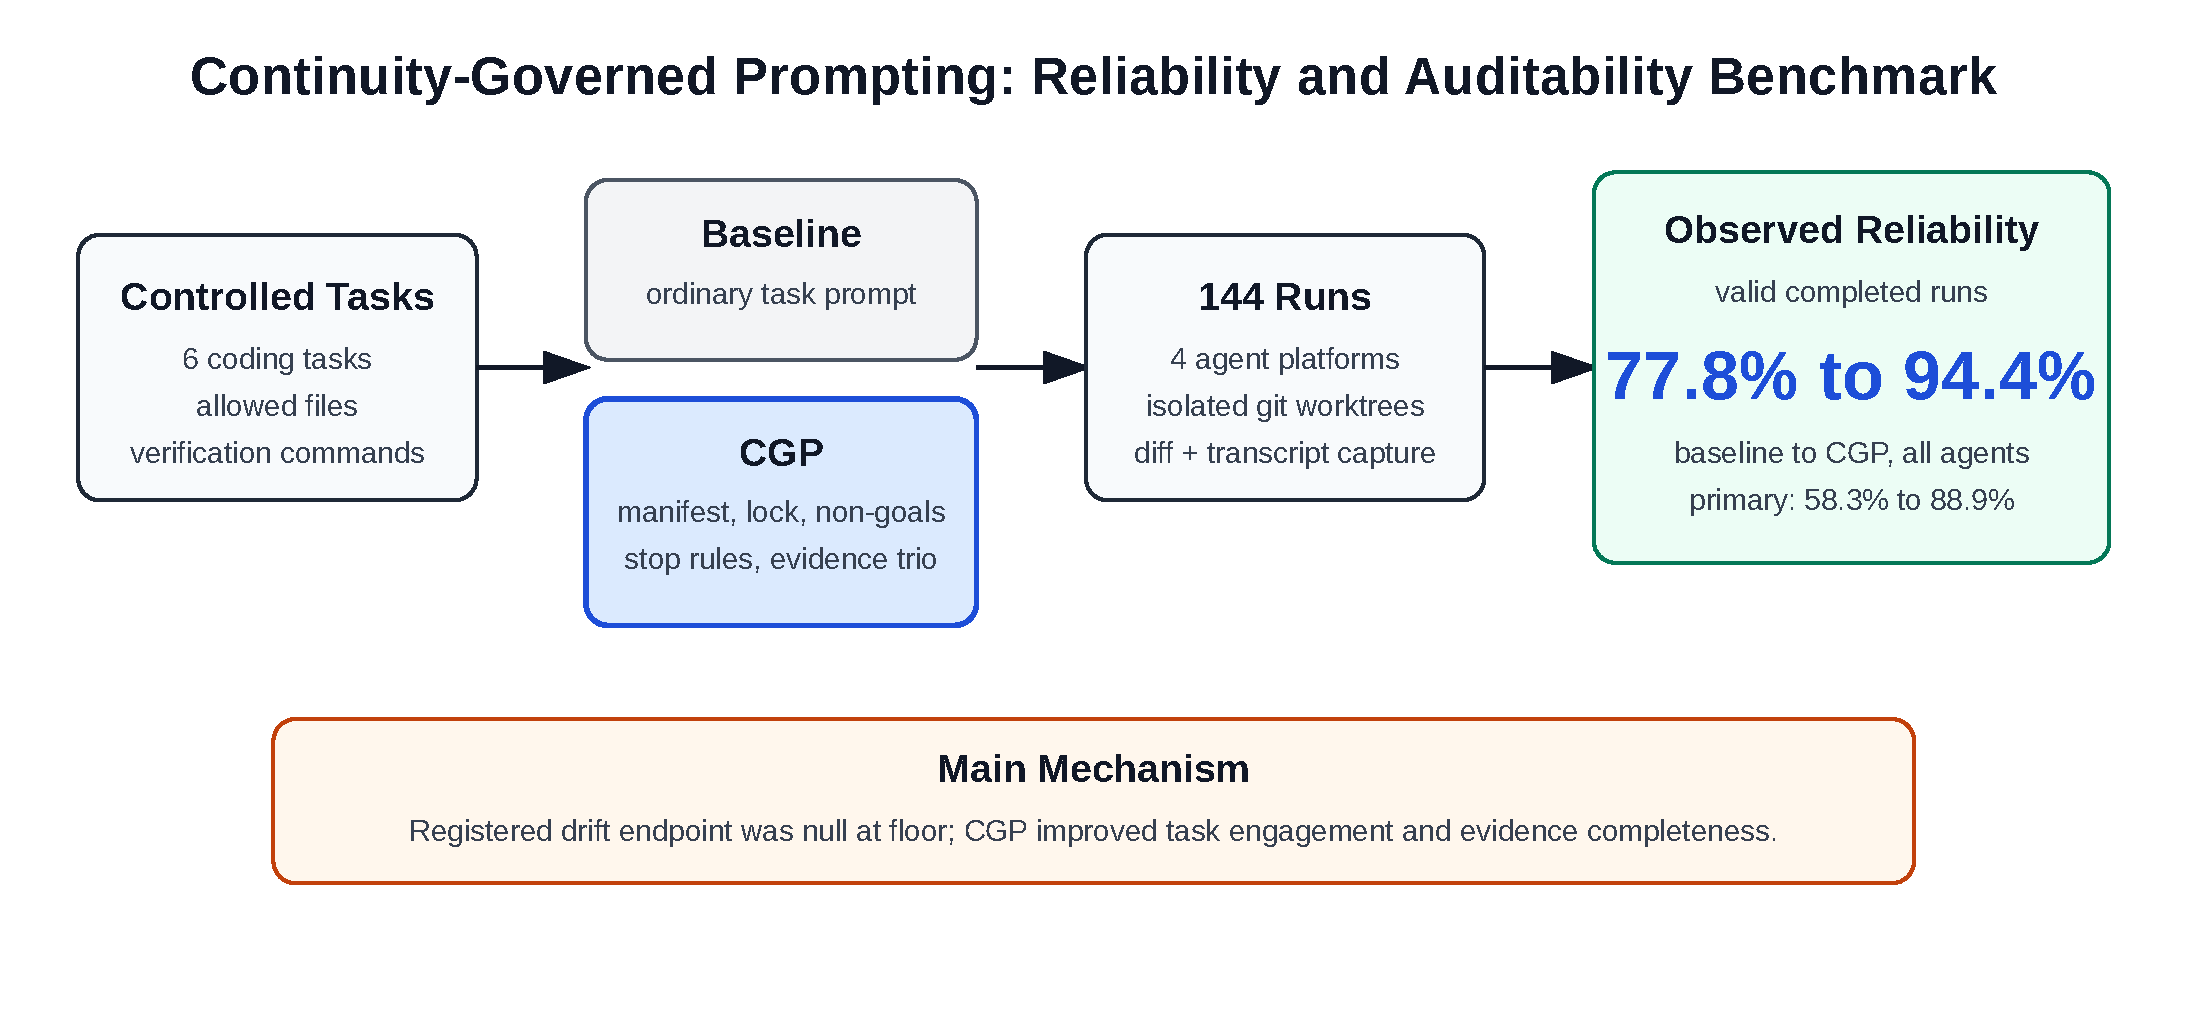
\includegraphics[width=0.92\textwidth]{graphical_abstract.pdf}
\caption*{Continuity-Governed Prompting reliability and auditability benchmark. The graphical abstract shows the controlled task set, the contrast between ordinary baseline prompting and the CGP scaffold, the isolated 144-run execution and capture process, and the observed operational validity movement from 77.8\% under baseline prompting to 94.4\% under CGP. The bottom panel states the governing interpretation boundary: the registered scope-drift endpoint was null at a baseline floor, while CGP improved task engagement and evidence completeness.}
\end{figure}


\section{Introduction}
Agent-assisted coding workflows increasingly depend on long-lived context, tool execution, repository state, and repeated handoffs between humans and models. Contemporary benchmarks have moved beyond isolated code generation toward repository-level and environment-interactive evaluations, including SWE-bench for real GitHub issues, SWE-agent for agent-computer interface design, SWE-Gym for software-engineering agent trajectories, MLE-bench for machine-learning engineering agents, and AgentBench for multi-environment agent evaluation (Jimenez et al., 2023; Yang et al., 2024; Pan et al., 2024; Chan et al., 2024; Liu et al., 2023). This shift reflects a practical reality: agent performance depends not only on model knowledge, but also on how the model is embedded in a work environment with files, commands, feedback, and persistent state.

In this setting, the central risk is not only whether an agent can solve a single isolated task, but whether it can remain bound to the intended objective, file boundary, verification requirement, and evidence record across operational steps. Prior agent methods such as ReAct, Reflexion, and Toolformer show that tool use, action traces, and feedback can improve agent behavior (Yao et al., 2022; Shinn et al., 2023; Schick et al., 2023). Continuity-Governed Prompting addresses a complementary problem. Rather than asking the model to internally reason better or self-reflect after failure, it imposes an external operational contract that defines the current task, permitted files, non-goals, verification gates, stop conditions, and evidence artifacts.

Continuity-Governed Prompting treats these failures as governance failures rather than merely prompt-quality failures. The method binds each run to an explicit active objective, allowed-file boundary, non-goals, stop condition, verification gate, and durable evidence record. In this study, the governance mechanism was implemented through a Next-Prompt Protocol scaffold that included a manifest, slice lock, active protocol, role context, and evidence trio. The purpose of the scaffold was not to make the coding task easier, but to make the operational contract harder to lose.

The preregistered primary hypothesis was that Continuity-Governed Prompting would reduce scope drift relative to ordinary baseline prompting. Additional registered hypotheses addressed handoff reproducibility and verification-command compliance. Because the experiment was run across multiple coding-agent systems, the study also evaluated whether continuity governance behaves as a portable control pattern or as an artifact of one model/tool implementation. The primary endpoint did not move in the favorable direction because baseline scope drift was absent in the primary dataset; that null result governs the interpretation of the study.

\section{Methods}
The benchmark used six controlled coding tasks in a small Python and JavaScript repository. The controlled repository was intentionally smaller than repository-scale benchmarks such as SWE-bench because the purpose of this experiment was not to measure frontier issue-resolution ability, but to isolate continuity-governance effects under repeatable conditions. Each task specified a description, allowed files, drift-surface files, and verification requirements. Runs were assigned to two prompt conditions. The baseline condition provided the task description, relevant files, and verification commands. The Continuity-Governed Prompting condition added the run-specific protocol scaffold, manifest, lock file, allowed-file boundary, non-goals, stop condition, and evidence-trio requirement.

The primary preregistered plan contained 72 planned runs: six tasks, two prompt conditions, two agent platforms, and three replications per task-condition-agent cell. The primary platforms were Claude Code and Aider. A companion extension added 72 planned runs using Codex and Gemini CLI with the same tasks, conditions, seed logic, and replication count. Primary and extension data were analyzed separately and together, with the extension interpreted as companion external-validity evidence rather than a silent replacement for the preregistered primary dataset.

Each run was executed in an isolated git worktree from the task start tag. The harness generated the prompt, executed the assigned agent, captured stdout and stderr or structured transcript output, computed a git diff against the run-specific metrics base commit, ran the task verification commands, and wrote raw artifacts under \texttt{runs/raw/RUN\_ID/}. For Continuity-Governed Prompting runs, the harness also copied the required evidence trio consisting of a design note, operational run record, and machine-readable evidence JSON file. Harness-defect and wrong-agent runs were preserved under \texttt{runs/raw/invalid/} and excluded from the planned-run analysis. The end-to-end capture flow is summarized in Figure 1.

\begin{figure}[H]\centering
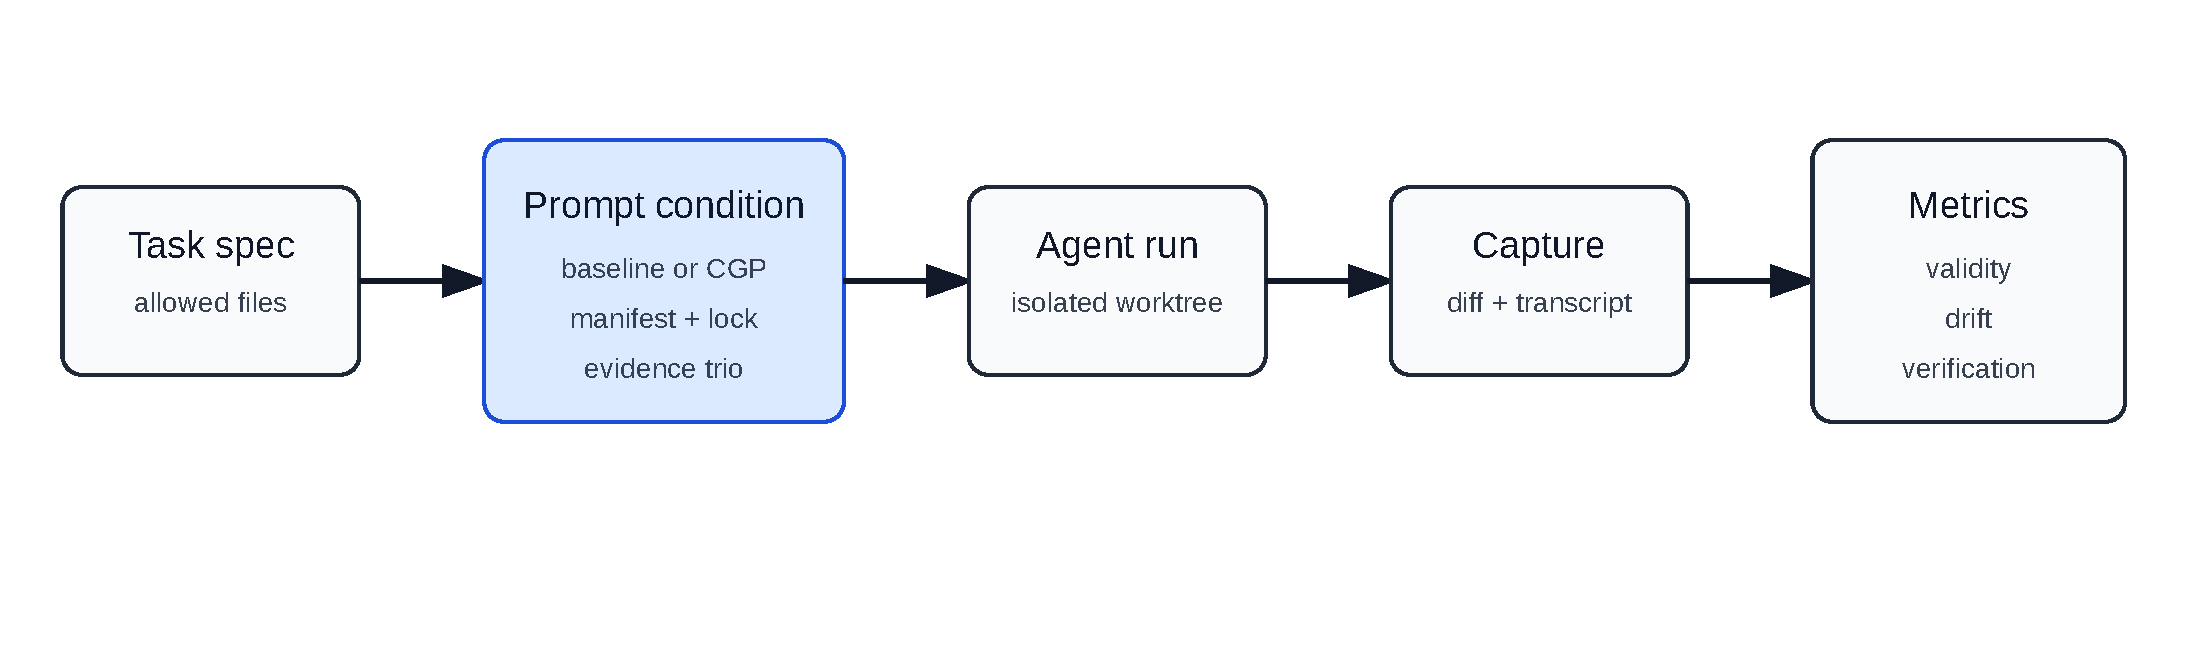
\includegraphics[width=0.92\textwidth]{figure1_benchmark_pipeline.pdf}
\caption{Benchmark run-capture pipeline. Each benchmark run began with a task specification containing allowed files and verification commands, then proceeded through either a baseline prompt or a CGP prompt that added manifest, lock, stop-condition, and evidence-trio requirements. Runs were executed in isolated git worktrees, captured as transcripts and diffs, and scored into run-level metrics. CGP evidence files were treated as allowed operational evidence when computing scope drift.}
\end{figure}


The registered primary endpoint for H1 was scope drift count. Scope drift was measured by comparing changed files against the task-specific allowed-file set, with CGP evidence files treated as allowed operational evidence. The registered analysis plan specified paired Wilcoxon signed-rank tests for M1 scope drift count and McNemar tests for M3 verification-command compliance and M5 task verification success. Exact tests were used in the final analysis because the event counts were sparse. The preregistration also specified M4 evidence-trio completeness as a CGP-only scaffold-adherence metric.

The manuscript additionally reports composite run validity because it is operationally important for deployment. A run was counted as valid when work was submitted, scope drift count was zero, verification passed, and, for Continuity-Governed Prompting runs, the evidence trio was complete. This composite was derived from captured run fields and is treated as an observed operational finding rather than as a registered confirmatory endpoint. Work submission and non-submission are likewise reported as operational findings because they explain a major failure mode but were not named as preregistered endpoints in the OSF preregistration packet. The epistemic boundary for these classifications is recorded in the preregistration deviation note, \texttt{docs/research\_integrity/CGP\_Benchmark\_Preregistration\_Deviation\_Note\_v1\_1.md}.

\section{Results}
The final planned-run analysis included 144 completed runs. The primary dataset contributed 72 runs, and the companion extension contributed 72 runs. Eight archived harness-defect records were preserved but excluded from the planned-run analysis.

Against the registered primary endpoint, the benchmark returned a null result at a baseline floor. In the primary preregistered dataset, baseline prompting produced 0 scope-drift events and Continuity-Governed Prompting produced 1 scope-drift event. The exact paired Wilcoxon two-sided p value was 1.0000. In the companion extension, baseline produced 1 scope-drift event and CGP produced 0, also with exact paired Wilcoxon two-sided p value 1.0000. Across all planned runs, baseline and CGP each produced 1 scope-drift event, and the exact paired Wilcoxon two-sided p value was 1.0000. The registered H1 claim is therefore not supported by this benchmark.

Verification-command compliance also did not improve in the primary dataset. Baseline compliance was 100.0\%, CGP compliance was 91.7\%, and the exact McNemar two-sided p value was 0.2500. Task verification success, a registered secondary metric, showed the same pattern in the primary dataset: 100.0\% under baseline and 91.7\% under CGP, with exact McNemar two-sided p = 0.2500. Across all planned runs, verification-command compliance and task verification success were both 100.0\% under baseline and 95.8\% under CGP, with exact McNemar two-sided p = 0.2500 for each metric. These registered and secondary tests do not support a favorable confirmatory effect.

The observed operational composite moved in the favorable direction. Across all agents and datasets, baseline prompting produced 56 valid runs out of 72, for a validity rate of 77.8\%. Continuity-Governed Prompting produced 68 valid runs out of 72, for a validity rate of 94.4\%. Work submission increased from 79.2\% under baseline prompting to 100.0\% under Continuity-Governed Prompting.

In the primary preregistered dataset, baseline prompting produced 21 valid runs out of 36, for a validity rate of 58.3\%. Continuity-Governed Prompting produced 32 valid runs out of 36, for a validity rate of 88.9\%. This contrast was driven largely by Aider and is limited to 18 runs per condition on that platform. Aider baseline runs were valid in 3 of 18 cases, whereas Aider CGP runs were valid in 14 of 18 cases. Claude Code completed all 36 primary runs validly across both conditions. Agent- and condition-level rates are reported in Table 1 and visualized in Figure 2.

\begin{table}[H]
\centering
\small
\resizebox{\textwidth}{!}{%
\begin{tabular}{llllllllll}
\toprule
Dataset & Agent & Condition & n & Valid n & Valid rate & Work submitted & Task success & Scope drift any & Evidence trio complete \\
\midrule
extension & codex & baseline & 18 & 18 & 100.0\% & 100.0\% & 100.0\% & 0.0\% & n/a \\
extension & codex & cgp & 18 & 18 & 100.0\% & 100.0\% & 100.0\% & 0.0\% & 100.0\% \\
extension & gemini-cli & baseline & 18 & 17 & 94.4\% & 100.0\% & 100.0\% & 5.6\% & n/a \\
extension & gemini-cli & cgp & 18 & 18 & 100.0\% & 100.0\% & 100.0\% & 0.0\% & 100.0\% \\
primary & aider & baseline & 18 & 3 & 16.7\% & 16.7\% & 100.0\% & 0.0\% & n/a \\
primary & aider & cgp & 18 & 14 & 77.8\% & 100.0\% & 83.3\% & 5.6\% & 94.4\% \\
primary & claude-code & baseline & 18 & 18 & 100.0\% & 100.0\% & 100.0\% & 0.0\% & n/a \\
primary & claude-code & cgp & 18 & 18 & 100.0\% & 100.0\% & 100.0\% & 0.0\% & 100.0\% \\
\bottomrule
\end{tabular}%
}
\caption{Summary by dataset, agent, and condition.}
\label{tab:summary}
\end{table}

\begin{figure}[H]\centering

\includegraphics[width=0.86\textwidth]{figure2_validity_by_agent_condition.png}
\caption{Operational run validity by agent and prompt condition. Bars show the proportion of runs classified as valid under the operational composite endpoint for each agent platform and prompt condition. This figure should not be interpreted as the registered primary drift endpoint; registered scope drift was analyzed separately and returned a null result at a baseline floor.}
\end{figure}


In the companion extension dataset, baseline prompting produced 35 valid runs out of 36, and Continuity-Governed Prompting produced 36 valid runs out of 36. Codex completed all baseline and governed extension runs validly. Gemini CLI completed all governed runs validly and had one invalid baseline run due to scope drift into \texttt{benchmark-repo/tests/test\_config.py}.

The dominant invalid-run mechanism was not broad file drift. Many Aider baseline runs submitted no work, producing no changed files while still passing the repository’s existing verification commands. These runs were classified as invalid in the operational composite because the assigned task was not performed. In contrast, CGP eliminated non-submission for Aider but did not eliminate all failures: several Aider CGP runs failed verification, and one had incomplete or misplaced evidence. Across all CGP runs, 71 of 72 had complete evidence trios, for a completeness rate of 98.6\%. Invalid-run mechanisms are summarized in Table 2 and Figure 3.

\begin{table}[H]
\centering
\small
\resizebox{\textwidth}{!}{%
\begin{tabular}{lllll}
\toprule
Dataset & Agent & Condition & Failure mechanism & n \\
\midrule
extension & gemini-cli & baseline & Scope drift & 1 \\
primary & aider & baseline & No work submitted & 15 \\
primary & aider & cgp & Scope drift & 1 \\
primary & aider & cgp & Verification failure & 3 \\
\bottomrule
\end{tabular}%
}
\caption{Invalid-run mechanisms.}
\label{tab:failures}
\end{table}

\begin{figure}[H]\centering
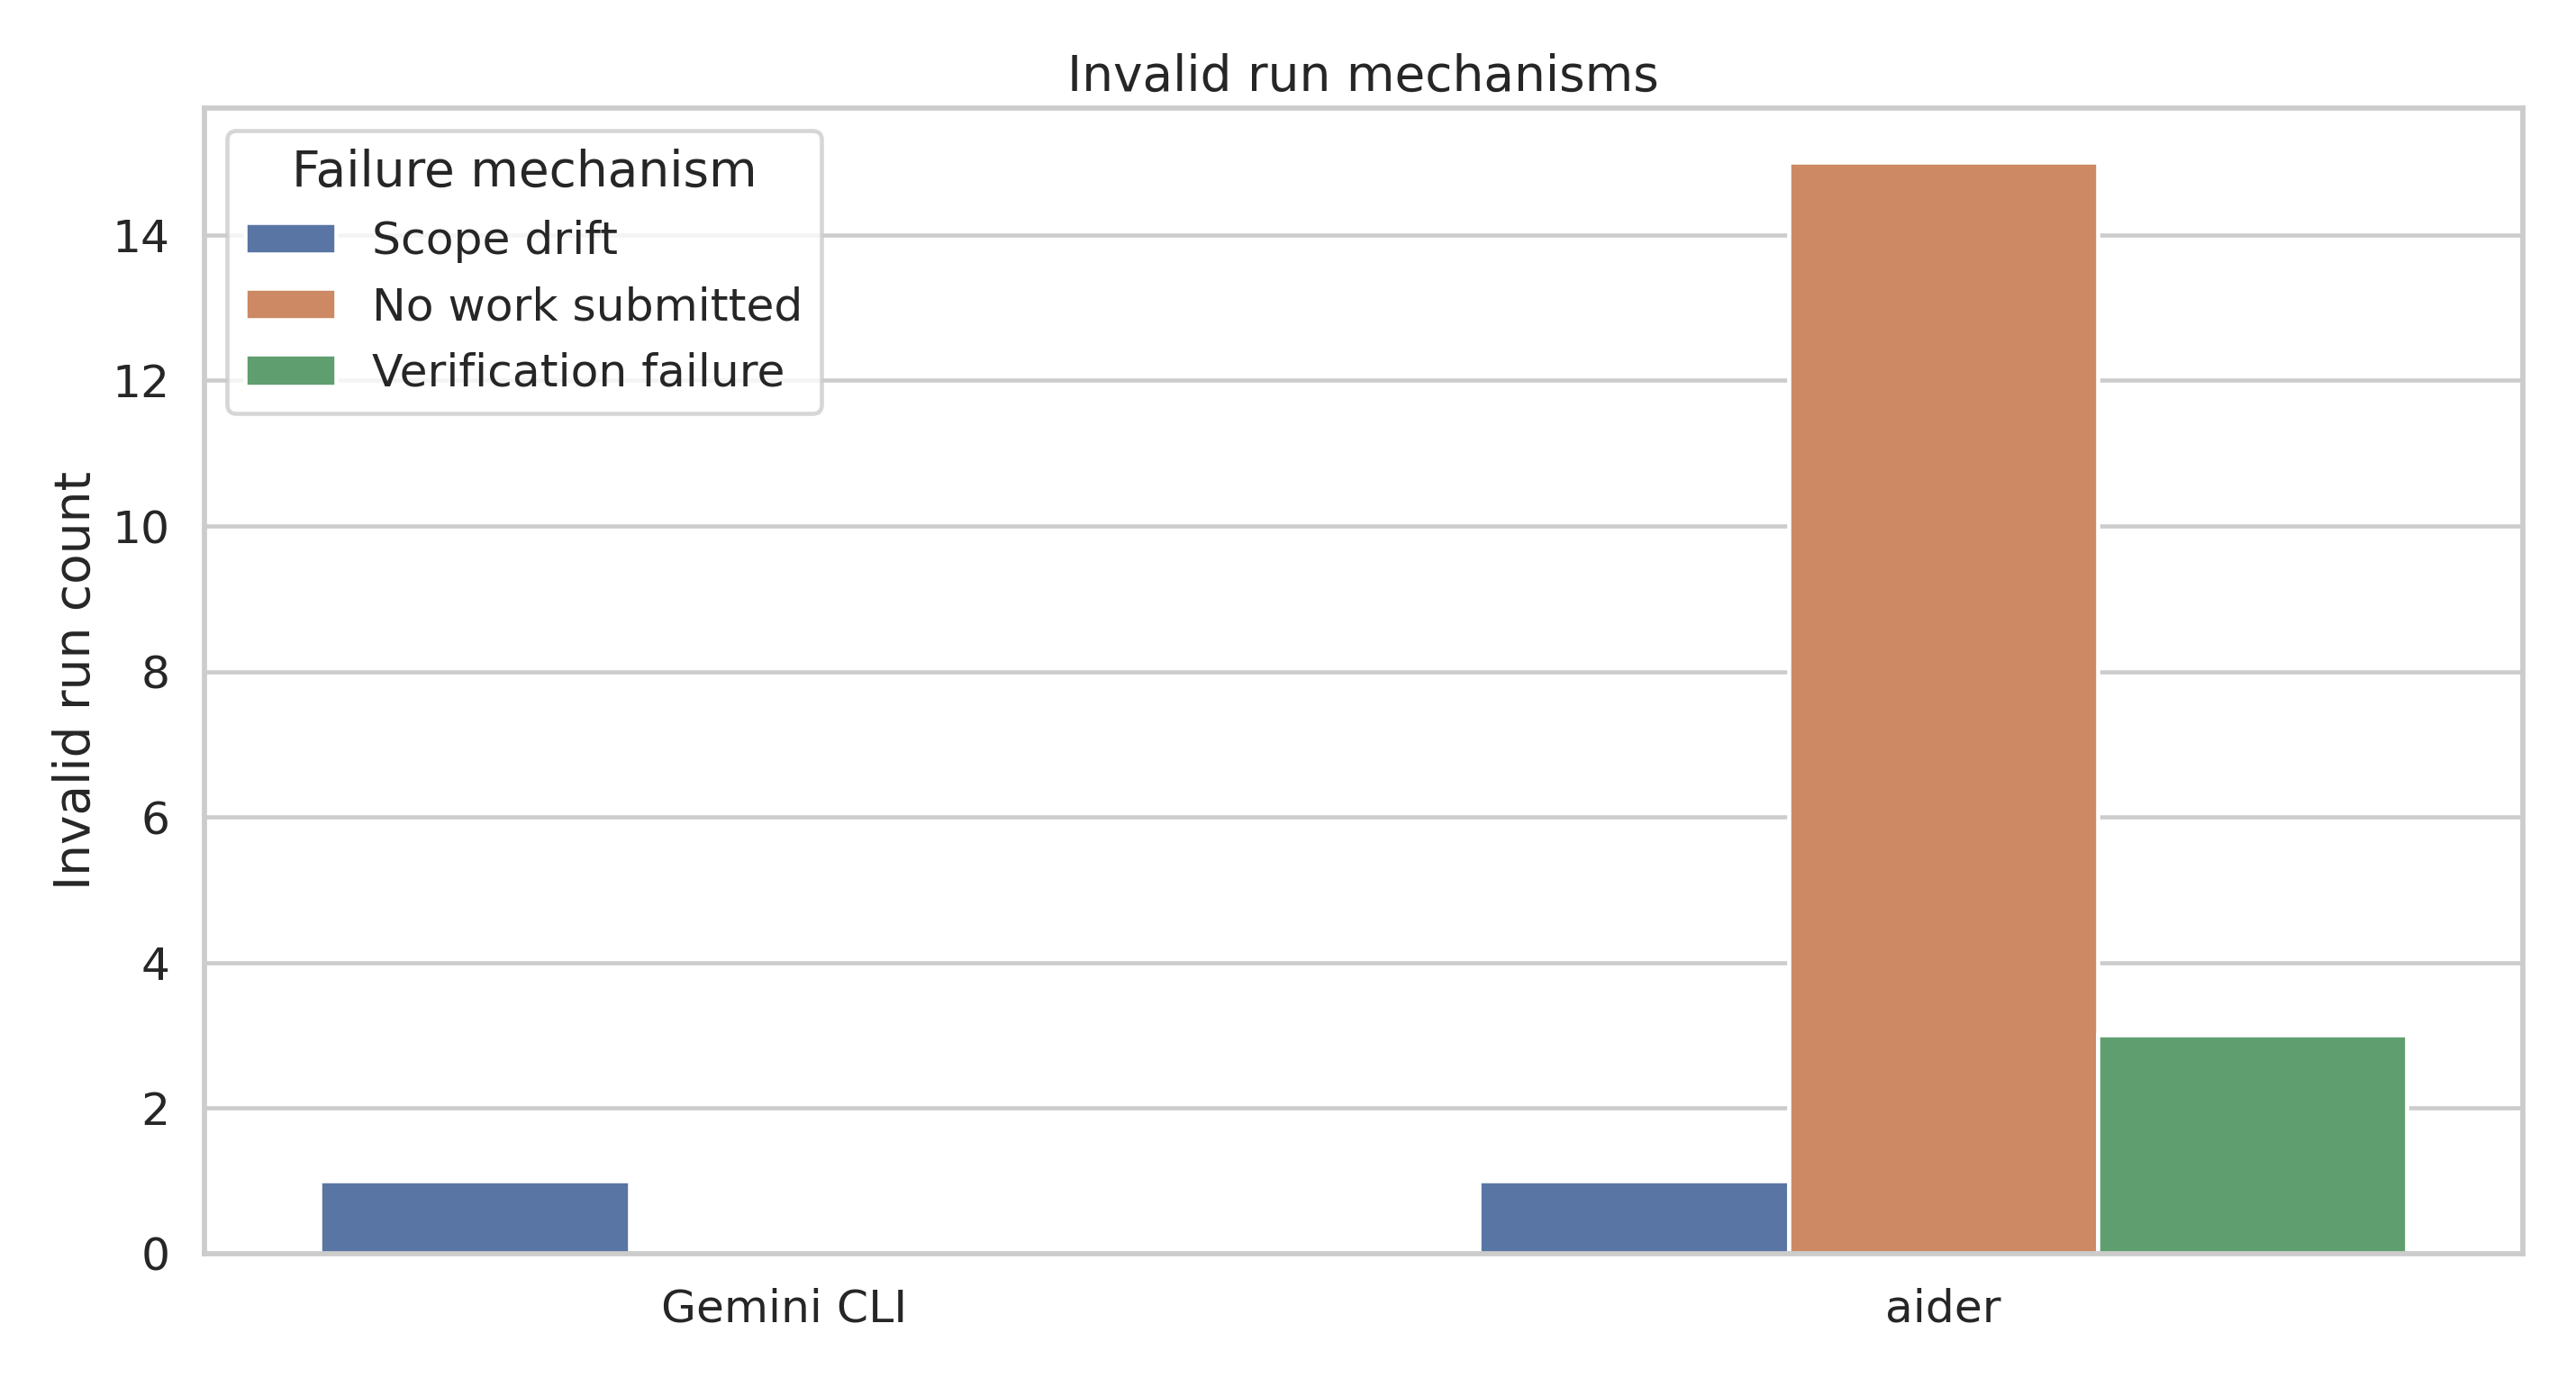
\includegraphics[width=0.86\textwidth]{figure3_invalid_run_mechanisms.png}
\caption{Invalid-run mechanisms by agent and prompt condition. Bars count invalid planned runs by observed failure mechanism. The dominant failure mode was non-submission in Aider baseline runs, where the agent completed without changing files while repository verification still passed.}
\end{figure}


\section{Discussion}
The results do not support the registered drift-reduction claim in this benchmark. The scope-drift endpoint was at a floor in the primary dataset, so the experiment could not demonstrate a reduction. Verification-command compliance also did not improve. The results do support a narrower operational claim: continuity governance can improve observed run validity, work submission, and evidence production in agent-assisted coding workflows. The mechanism was especially visible in Aider: baseline prompting frequently produced no submitted work, whereas the governed prompt reliably induced task action and evidence generation. This suggests that governance scaffolds can improve execution commitment and auditability in agents that may otherwise terminate without making task changes.

The study also shows that the governance effect is platform-dependent. Claude Code and Codex performed at ceiling in both conditions, leaving little room for improvement. Gemini CLI was also near ceiling, with one baseline drift event and no governed drift events. These results are consistent with broader agent-evaluation work showing that environment and scaffold design can materially shape agent behavior (Yang et al., 2024; Liu et al., 2023). They also limit the claim: the measurable benefit depends on the agent’s baseline reliability and failure modes. In high-performing agents, CGP may primarily add auditability and evidence structure. In agents with weaker baseline task persistence, CGP may materially improve run validity.

The findings should be interpreted with several limitations. The registered endpoint suffered a floor effect, with no baseline scope drift in the primary dataset. Three of four evaluated platforms were at or near ceiling, and the largest validity contrast was concentrated in one platform. The benchmark repository was controlled and artificial, which improves measurement precision but limits direct generalization to large production repositories. The validity definition intentionally combines task action, scope control, verification success, and evidence completeness, so it is an operational composite rather than a pure measure of code correctness. Because composite validity and work submission were not named as preregistered endpoints, they should be treated as operational findings that motivate future confirmatory work rather than as confirmatory hypothesis tests. Some invalid baseline runs passed verification because the existing test suite did not detect omitted docstring or implementation work. This is not a scoring error; it reflects a real limitation of verification-only success criteria and supports the value of explicit work-submission and evidence checks.

Future work should extend the benchmark to larger repositories, additional task types, and longer multi-turn handoffs, including tasks engineered to produce measurable baseline drift if the drift-reduction hypothesis is to be tested directly. A further analysis should model agent platform explicitly rather than aggregating across systems, because the observed failure modes differed substantially by agent. The most immediate practical implication is that organizations adopting coding agents should treat continuity governance as an operational control layer: a way to bind agent work to explicit state, scope, verification, and durable evidence rather than relying on conversational summaries alone.

\section{Declarations}
The study was preregistered on OSF at \texttt{https://osf.io/fnmg5}. After analysis, the authors added a preregistration deviation note documenting that the registered primary endpoint, scope drift count, returned a null result at a baseline floor and distinguishing confirmatory registered endpoints from observed operational findings. The governing deviation note is stored in the repository as \texttt{docs/research\_integrity/CGP\_Benchmark\_Preregistration\_Deviation\_Note\_v1\_1.md}.

All benchmark code, task specifications, runner scripts, raw planned-run records, archived invalid harness records, processed metrics, registered-analysis outputs, figures, and manuscript materials are available in the public repository \texttt{https://github.com/heart-ai-foundation/cgp-benchmark}. The processed analysis files used for the manuscript are stored under \texttt{runs/processed/}; the registered-analysis outputs are \texttt{runs/processed/registered\_analysis.md} and \texttt{runs/processed/registered\_analysis.json}.

The author developed Continuity-Governed Prompting and may have a financial interest through future commercial implementation services offered separately by HeartCore Ventures LLC. The methodology, benchmark repository, preregistration materials, deviation note, and manuscript materials are published by the Heart AI Foundation with the dual-entity boundary disclosed in the research-integrity record.

AI language models were used to assist with drafting, code execution, benchmark operation, analysis scripting, and manuscript revision. Experimental design decisions, interpretation boundaries, claims governance, and final responsibility for the manuscript remain with the author.


\clearpage
\section*{References}
\begin{enumerate}
\item Chan, J. S., Chowdhury, N., Jaffe, O., Aung, J., Sherburn, D., Mays, E., Starace, G., Liu, K., Maksin, L., Patwardhan, T., Weng, L., \& Mądry, A. (2024). \textit{MLE-bench: Evaluating machine learning agents on machine learning engineering}. arXiv:2410.07095. \url{https://arxiv.org/abs/2410.07095}
\item Jimenez, C. E., Yang, J., Wettig, A., Yao, S., Pei, K., Press, O., \& Narasimhan, K. (2023). \textit{SWE-bench: Can language models resolve real-world GitHub issues?} arXiv:2310.06770. \url{https://arxiv.org/abs/2310.06770}
\item Liu, X., Yu, H., Zhang, H., Xu, Y., Lei, X., Lai, H., Gu, Y., Ding, H., Men, K., Yang, K., Zhang, S., Deng, X., Zeng, A., Du, Z., Zhang, C., Shen, S., Zhang, T., Su, Y., Sun, H., Huang, M., Dong, Y., \& Tang, J. (2023). \textit{AgentBench: Evaluating LLMs as agents}. arXiv:2308.03688. \url{https://arxiv.org/abs/2308.03688}
\item Pan, J., Wang, X., Neubig, G., Jaitly, N., Ji, H., Suhr, A., \& Zhang, Y. (2024). \textit{Training software engineering agents and verifiers with SWE-Gym}. arXiv:2412.21139. \url{https://arxiv.org/abs/2412.21139}
\item Schick, T., Dwivedi-Yu, J., Dessì, R., Raileanu, R., Lomeli, M., Zettlemoyer, L., Cancedda, N., \& Scialom, T. (2023). \textit{Toolformer: Language models can teach themselves to use tools}. arXiv:2302.04761. \url{https://arxiv.org/abs/2302.04761}
\item Shinn, N., Cassano, F., Berman, E., Gopinath, A., Narasimhan, K., \& Yao, S. (2023). \textit{Reflexion: Language agents with verbal reinforcement learning}. arXiv:2303.11366. \url{https://arxiv.org/abs/2303.11366}
\item Yang, J., Jimenez, C. E., Wettig, A., Lieret, K., Yao, S., Narasimhan, K., \& Press, O. (2024). \textit{SWE-agent: Agent-computer interfaces enable automated software engineering}. arXiv:2405.15793. \url{https://arxiv.org/abs/2405.15793}
\item Yao, S., Zhao, J., Yu, D., Du, N., Shafran, I., Narasimhan, K., \& Cao, Y. (2022). \textit{ReAct: Synergizing reasoning and acting in language models}. arXiv:2210.03629. \url{https://arxiv.org/abs/2210.03629}
\end{enumerate}

\end{document}
